%!TEX encoding = UTF-8 Unicode
%!TEX root = ../doc-plm.tex


\chapter{Introduction}

%--- Pour supprimer tout en-tête et pied de page sur la 1re page d'un chapitre
\thispagestyle{empty}



\section{Cible}




\chapter{Déclaration des registres}

La déclaration d'un registre obéit à une syntaxe particulière, ne serait-ce que parce que son adresse absolue doit y être spécifiée. Pour de nombreux registres, un bit ou un groupe de bits ont une signification particulière, et obtenir la valeur d'un champ ou modifier sa valeur est une opération courante.

À titre d'exemple, nous allons nous intéresser au registre \texttt{SYS\_CSR} du processeur ARMv7-M. Le \emph{manuel de référence de l'architecture ARMv7-M}\footnote{\url{http://infocenter.arm.com/help/index.jsp?topic=/com.arm.doc.ddi0403e.b/index.html}} décrit ce registre comme indiqué à la \refFigure{}{definitionSystick}. Cette description indique l'adresse du registre (\texttt{0xE000E010}), et les différents champs qui le composent.

\begin{figure}[t]
\centering
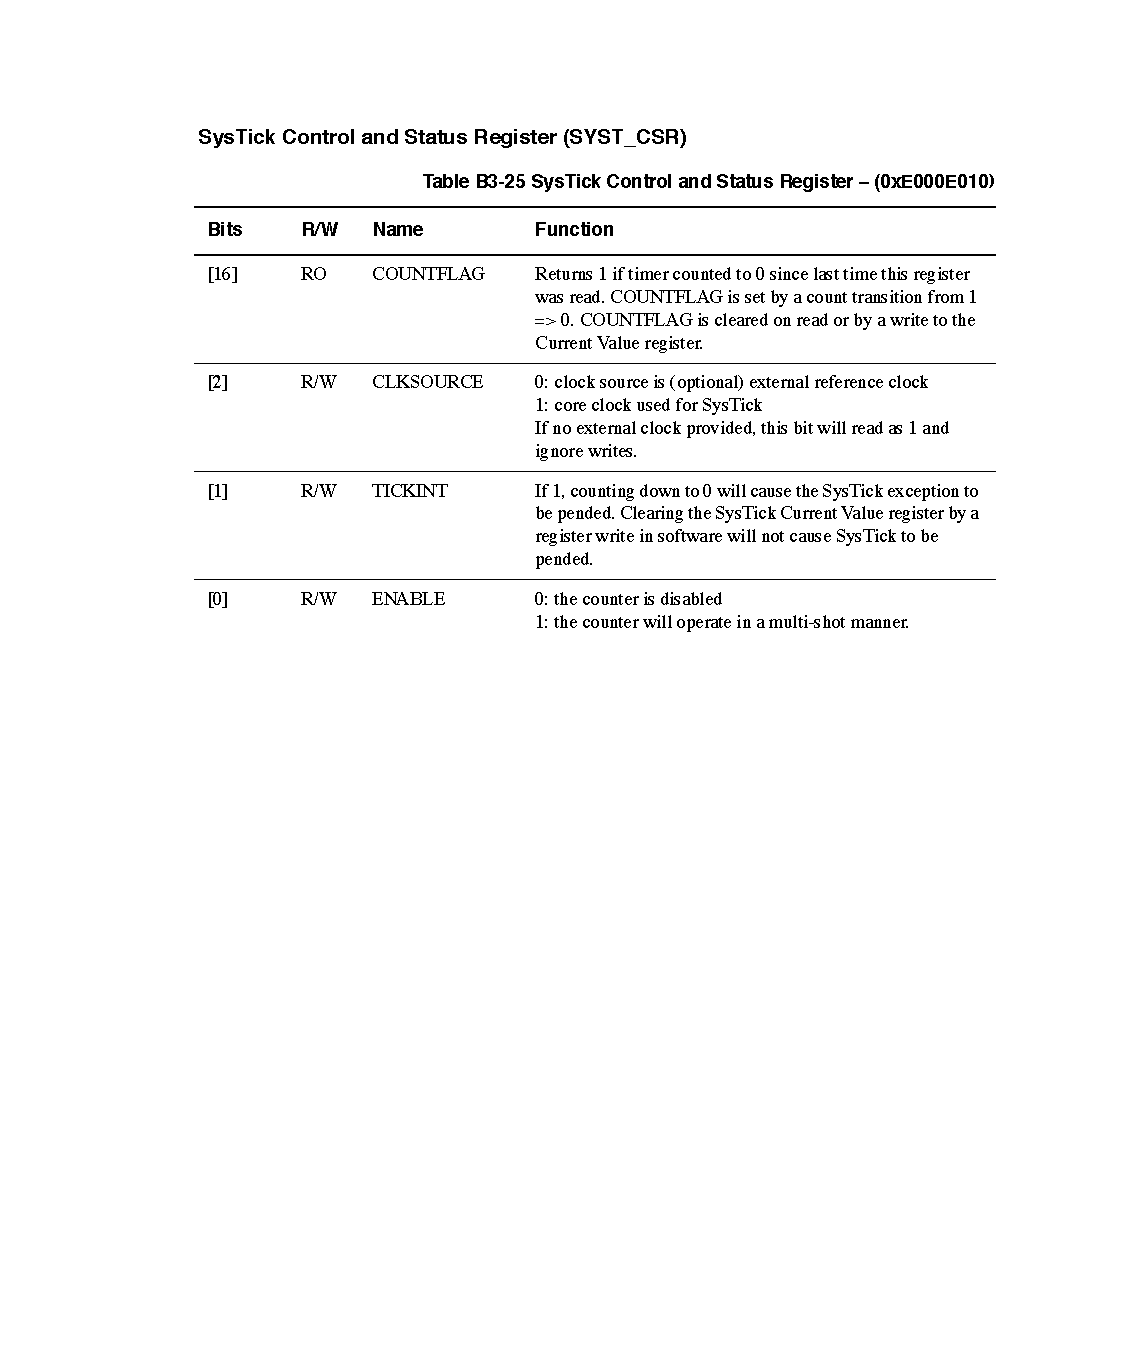
\includegraphics{chapitres/arm-v7-systick.pdf}
\caption{Registre de contrôle \texttt{SYS\_CSR} intégré dans l'ARMv7}
\labelFigure{definitionSystick}
\ligne
\end{figure}




\section{Simple déclaration d'un registre}
Pour déclarer le registre \texttt{SYS\_CSR} (\refFigure{}{definitionSystick}), on écrira simplement :
\begin{PLM}
register SYS_CSR at 0xE000_E010 : UInt32
\end{PLM}

Le type \plm+UInt32+ qui est mentionné signifie que les valeurs écrites et lues de ce registre sont des entiers non signés de 32 bits. Tout type entier, signé ou non signé est autorisé.

Pour lire ou écrire ce registre, on le nomme comme s'il s'agissait d'une simple variable. Par exemple, pour activer le comptage du \emph{Systick Timer} et l'interruption correspondante, il faut mettre à $1$ les bits \texttt{CLKSOURCE}, \texttt{TICKINT} et \texttt{ENABLE}. On écrit donc :
\begin{PLM}
SYST_CSR = (1 << 2) | (1 << 1) | (1 << 0)
\end{PLM}

Pour savoir si le bit \texttt{TICKINT} est activé, on écrit :
\begin{PLM}
let tickIntActif : Bool = (SYST_CSR & (1 << 1)) != 0
\end{PLM}

Ces écritures peuvent être rendues plus intelligibles en précisant la composition du registre \texttt{SYS\_CSR} dans sa déclaration. C'est ce qui va être réalisé dans la section suivante.


\section{Déclaration d'un registre et de ses champs}

%\noindent{\setlength\fboxsep{4pt}\fcolorbox{gray}{green!25!blue!10}{
%\begin{minipage}{0.96\linewidth}
%Peut être qualifiée de\, \index{Temps réel!définition|textbf}\emph{temps réel}\,
% une application informatique qui produit des résultats dont la validité ne dépend pas que de la justesse de leurs valeurs, mais aussi de la date de leur production : un résultat juste ne sera valide que s'il est délivré dans une fenêtre temporelle spécifiée.
%\end{minipage}}}


Il est possible de préciser la composition des champs entiers et booléens d'un registre :
\begin{PLM}
register SYS_CSR at 0xE000_E010
  : UInt32 {15, COUNTFLAG, 13, CLKSOURCE, TICKINT, ENABLE}
\end{PLM}

Cette écriture n'est autorisée que si le type nommé (ici \plm+UInt32+) est une type entier non signé. Les types signés (\plm+Int32+, ...) sont interdits. Entre accolades, est décrite la composition du registre, bit par bit, en commençant par le poids fort. Un nombre entier signifie un nombre de bits inutilisés ; un identificateur nomme un bit particulier. Cette description correspond à celle de la \refFigure{}{definitionSystick} :
\begin{itemize}
\item les 15 bits de poids fort sont inutilisés ;
\item le bit 16 est le bit \texttt{COUNTFLAG} ;
\item les 13 bits suivants sont inutilisés ;
\item les bits 2, 1 et 0 sont respectivement \texttt{CLKSOURCE}, \texttt{TICKINT} et \texttt{ENABLE}
\end{itemize}

Le compilateur vérifie que la description des champs définit exactement le nombre de bits du type nommé, ici les 32 bits du type \plm+UInt32+.


\subsection{Constantes associées aux champs booléens}

Le délimiteur \plm+::+ permet de définir des constantes correspondant aux bits d'un registre. Par exemple :
\begin{PLM}
SYST_CSR::CLKSOURCE // De type UInt32, égal à 4
\end{PLM}
Ces constantes ont le type du registre nommé.

Ainsi, pour activer le comptage du \emph{Systick Timer} et l'interruption correspondante, il faut mettre à $1$ les bits \texttt{CLKSOURCE}, \texttt{TICKINT} et \texttt{ENABLE}. On écrit donc :
\begin{PLM}
SYST_CSR = SYST_CSR::CLKSOURCE | SYST_CSR::TICKINT | SYST_CSR::ENABLE
\end{PLM}


\subsection{Accès en lecture}
Pour accéder à la valeur d'un champ, on utilise la notation pointée en nommant ce champ :
\begin{PLM}
let x : UInt32 = SYS_CSR.CLKSOURCE // 0 ou 4
\end{PLM}
Ceci effectue simplement un masquage de façon à isoler le bit demandé. Aucun décalage n'est réalisé. Comme le bit \texttt{CLKSOURCE} est le 2\up{e}, le résultat est \plm+0+ ou \plm+4+. Le type de l'expression \plm+SYS_CSR.CLKSOURCE+ est le type du registre \plm+SYS_CSR+, donc \plm+UInt32+.

Si l'on veut obtenir un résultat justifié à droite, on utilise en plus l'accesseur \plm+.shift+ :
\begin{PLM}
let x : UInt32 = SYS_CSR.CLKSOURCE.shift // 0 ou 1
\end{PLM}

L'accesseur  \plm+.bool+ permet d'obtenir une valeur booléenne correspondant à la valeur d'un bit d'un registre :
\begin{PLM}
let x : Bool = SYS_CSR.CLKSOURCE.bool // false ou true
\end{PLM}




\section {Champs entiers}

L'accès à un champ s'effectue par la notation pointée \plm+.+. Par exemple :
\begin{PLM}
PORTA_PCR0.mux
\end{PLM}

renvoie un \plm+UInt32+ valant \plm+0+, \plm+0x100+, \plm+0x200+, ..., \plm+0x700+.

Pour obtenir une valeur justifiée à droite, on ajoute l'accesseur \plm+.shift+ :
\begin{PLM}
PORTA_PCR0.mux.shift
\end{PLM}

La valeur renvoyée est alors comprise en \plm+0+ et \plm+7+.

\section{Attribut \texttt{@ro}}
Un registre accepte l'attribut \plm+@ro+, qui signifie qu'il est en lecture seule. Par exemple :
\begin{PLM}
register @ro nom_registre at 0x1234 : UInt32
\end{PLM}

Toute tentative de faire figurer ce registre dans une construction qui provoque une écriture de celui-ci entraîne l'apparition d'une erreur de compilation.

